\chapter{Reta Projetiva} \label{chap:retaprojetiva}

\section{Definição} \label{sec:defnretaprojetiva}

\begin{defn}[Reta Projetiva Real] \label{defn:retaprojetivareal}
A \emph{reta projetiva real \(\mathbb{P}^1(\mathbb{R})\)} é o conjunto das retas do \(\mathbb{R}^2\) que passam pela origem.
Elementos da reta projetiva real são chamados de \emph{pontos projetivos}.
\end{defn}

\begin{figure}[hbtp]
  \centering
  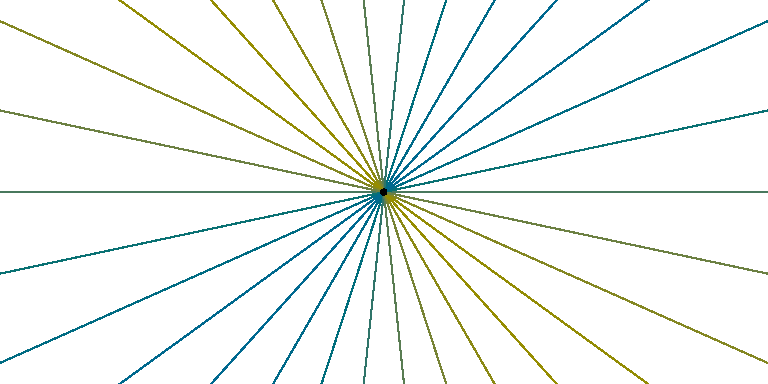
\includegraphics{figures/retaprojetiva.pdf}
  \caption{Reta Projetiva Real}
\end{figure}

Como um abuso de notação, chamaremos a reta projetiva real somente de reta projetiva.
Quando o significado estiver claro, podemos chamar a reta projetiva de reta, e o ponto projetivo de ponto.

Em termos de Álgebra Linear, os pontos da reta projetiva são os subespaços do $\mathbb{R}^2$ com dimensão~$1$.

Podemos inferir uma representação dos pontos projetivos da reta projetiva a partir dos vetores do \(\mathbb{R}^2\).
Se \(\mathbf{v} \neq (0, 0)\), vamos chamar de \([\mathbf{v}]\) a única reta que passa pela origem e por \(\mathbf{v}\).
Lembre-se que uma reta no \(\mathbb{R}^2\) é definida por dois pontos distintos; portanto, a reta \([\mathbf{v}]\) está bem definida.

De modo mais preciso, podemos concluir que \([\mathbf{v}]\) é o conjunto dos múltiplos reais de \(\mathbf{v}\), isto é, é o conjunto \(\{ \lambda \mathbf{v} : \lambda \in \mathbb{R}\}\).

Porém, essa representação não é única.
Por exemplo, \([(1, 2)]\), \([(2, 4)]\) e \([(-1, -2)]\) representam o mesmo ponto projetivo, isto é, a mesma reta.
De modo geral, se \(\lambda \neq 0\), os pontos projetivos \([\mathbf{v}]\) e \([\lambda \mathbf{v}]\) são os mesmos.

Apesar da representação não ser única, temos que \([\mathbf{v}] = [\mathbf{u}]\) se, e somente se, \(\mathbf{u}\) é um múltiplo real de \(\mathbf{v}\).
Em outras palavras, \([\mathbf{v}] = [\mathbf{u}]\) se, e somente se, existe \(\lambda \in \mathbb{R}\) tal que \(\mathbf{u} = \lambda\mathbf{v}\).

Portanto, o sistema de coordenadas da reta projetiva é um pouco diferente do sistema que estamos acostumados, mas continua sendo útil mesmo assim.
Chamamos sistemas como esse, em que múltiplicar por um escalar não muda o ponto, de \emph{sistema de coordenadas homogêneas}.

\begin{exmp}
Os pontos projetivos $[1,0]$, $[0,1]$, $[1,1]$ e $[2,1]$ correspondem respectivamente ao eixo $x$, ao eixo $y$, à reta $y=x$ e à reta $y=\frac{1}{2}x$ do $\mathbb{R}^2$.
\end{exmp}

Por que chamamos a reta projetiva de ``reta''? Uma maneira de responder essa pergunta é, dada uma base do $\mathbb{R}^2$, considerar a reta $y=1$.
Note que essa reta não é um ponto projetivo, pois não passa pela origem. Com isso, podemos tomar como representante, para cada ponto projetivo, sua interseção com a reta $y=1$.

\begin{figure}[hbtp]
  \centering
  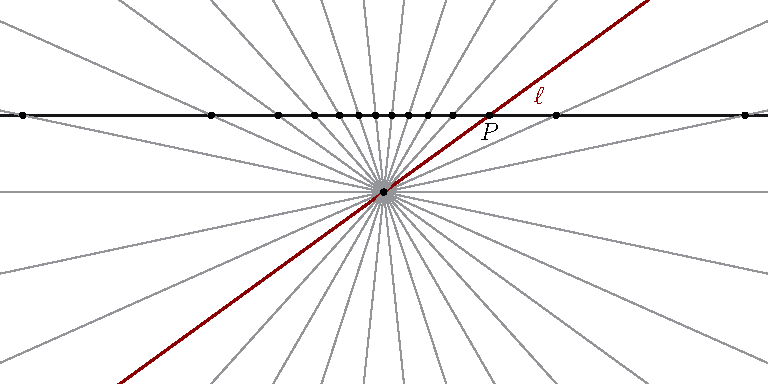
\includegraphics{figures/retaprojetivaretay1.pdf}
  \caption{Reta Projetiva Real e reta \(y = 1\)}
\end{figure}

Contudo, vemos que exatamente um dos pontos projetivos, a reta \(y = 0\), não intersecta a reta \(y = 1\).
Para essa reta, vamos escolher o representante $[(1,0)]$.
Portanto, 
\begin{equation} \label{eqn:retaprojetivaretaponto}
	\mathbb{P}^1(\mathbb{R}) = \{ [(x,1)] : x \in \mathbb{R} \} \cup \{[(1,0)]\},
\end{equation}
ou seja, podemos interpretar reta projetiva real como uma reta real com um ponto extra.

\section{Mudança de Base}

No \(\mathbb{R}^2\), temos liberdade para escolher dois vetores (linearmente independentes) \(\mathbf{v_1}\) e \(\mathbf{v_2}\) e chamá-los de \((1, 0)\) e \((0, 1)\), respectivamente.
Feito isso, todos os outros vetores do \(\mathbb{R}^2\) estão unicamente definidos.

Na reta projetiva, podemos fazer algo parecido. Dados dois pontos projetivos \(A = [\mathbf{v_1}]\) e \(B = [\mathbf{v_2}]\), podemos escolher uma base para o \(\mathbb{R}^2\) de modo que \(\mathbf{v_1}\) e \(\mathbf{v_2}\) são representados por \((1, 0)\) e \((0, 1)\), respectivamente.
Desse modo, \(A = [(1, 0)]\) e  \(B = [(0, 1)]\).

Porém, se tivéssemos escolhido a base do \(\mathbb{R}^2\) para serem os vetores \(3\mathbf{v_1}\) e  \(5\mathbf{v_2}\); também concluiríamos que \(A = [(1, 0)] \) e \(B = [(0, 1)]\). Parece que temos mais liberdade na reta projetiva do que em \(\mathbb{R}^2\). Com isso, estamos prontos para o primeiro teorema sobre a reta projetiva.

\begin{thm}\label{thm:trespontos}
  Dados três pontos projetivos distintos \(A\), \(B\) e \(C\), podemos escolher uma base apropriada do \(\mathbb{R}^2\) para a qual \(A = [(1, 0)]\),  \(B = [(0, 1)]\) e \(C = [(1, 1)]\).
\end{thm}
\begin{proof}
  Existem vetores \(\mathbf{v_1}\), \(\mathbf{v_2}\) e \(\mathbf{v_3}\) no \(\mathbb{R}^2\) para os quais \(A = [\mathbf{v_1}]\), \(B = [\mathbf{v_2}]\) e \(C = [\mathbf{v_3}]\).

  Considere a base \(\beta = \{\mathbf{v_1}, \mathbf{v_2}\}\) do \(\mathbb{R}^2\). Nessa base, \(A = [(1, 0)]\),  \(B = [(0, 1)]\) e \(C = [(\lambda, 1)]\), para algum \(\lambda \in \mathbb{R}\).

  Considere a base \(\gamma = \{\lambda\mathbf{v_1}, \mathbf{v_2}\}\) do \(\mathbb{R}^2\). Nessa segunda base, \(A = [(1, 0)]\),  \(B = [(0, 1)]\) e \(C = [(1, 1)]\), como desejado.
\end{proof}

\section{Razão Cruzada}

Nessa seção, vamos deixar o Teorema \ref{thm:trespontos} um pouco mais forte: se adicionarmos um quarto ponto projetivo \(D\), a representação dele em coordenadas estará unicamente definida (ignorando multiplicação por escalar).

Como abuso de notação, escreveremos \([a, b]\) para querer dizer \([(a, b)]\). É importante lembrar que essa representação depende da base escolhida para \(\mathbb{R}^2\).

\begin{thm}\label{thm:trespontosdefinem}
  Dados quatro pontos projetivos distintos \(A\), \(B\), \(C\) e \(D\), existe um único \(d \in \mathbb{R}\) tal que, se \(\beta\) é uma base do \(\mathbb{R}^2\) satisfazendo \(A = [1, 0]\), \(B = [0, 1]\) e \(C = [1, 1]\), então \(D = [d, 1]\).
\end{thm}
\begin{proof}
  Suponha que \(\beta = \{\mathbf{v_1}, \mathbf{v_2}\}\) e \(\gamma = \{\mathbf{u_1}, \mathbf{u_2}\}\) são bases de \(\mathbb{R}\) satisfazendo as condições, isto é, tais que
  \begin{align}
    A &= [\mathbf{v_1}] = [\mathbf{u_1}], \\
    B &= [\mathbf{v_2}] = [\mathbf{u_2}], \\
    C &= [\mathbf{v_1} + \mathbf{v_2}] = [\mathbf{u_1} + \mathbf{u_2}].
  \end{align}

  Isso implica que existem constantes reais \(a, b, c\) tais que
  \begin{align}
    \mathbf{u_1} &= a \mathbf{v_1}, \\
    \mathbf{u_2} &= b \mathbf{v_2}, \\
    \mathbf{u_1} + \mathbf{u_2} &= c \left(\mathbf{v_1} + \mathbf{v_2}\right).
  \end{align}

  Note que \((a - c)\mathbf{v_1} + (b - c)\mathbf{v_2} = \mathbf{0}\) e, como \(\mathbf{v_1}\), \(\mathbf{v_2}\) são linearmente independentes, temos que \(a = b = c\).

  Finalmente, se \(D = [d\mathbf{v_1} + \mathbf{v_2}]\), concluímos que \(D = [a\left(d\mathbf{v_1} + \mathbf{v_2}\right)] = [d\mathbf{u_1} + \mathbf{u_2}]\). Portanto, \(D = [d, 1]\) em ambas as bases \(\beta\) e \(\gamma\); ou seja, independentemente da base, \(d\) está unicamente definido.
\end{proof}

\begin{defn}[Razão Cruzada]\label{defn:razaocruzada}
  Dados quatro pontos projetivos \(A\), \(B\), \(C\) e \(D\), a \emph{razão cruzada dos pontos \(A\), \(B\), \(C\) e \(D\)}, denotada por \((A, B; C, D)\) é definida pelo número real \(d\) achado no Teorema \ref{thm:trespontosdefinem}.
\end{defn}

\begin{prop}
  Se \((A, B; C, D) = (A, B; C, E) = d\), então  \(D = E\).
\end{prop}
\begin{proof}
  Escolha a base \(\beta\) como descrita no Teorema \ref{thm:trespontosdefinem}. Ambos pontos \(D\) e \(E\) são \([d, 1]\) na base \(\beta\); consequentemente \(D = E\).
\end{proof}

\begin{exer}
Dada uma base \(\beta\) do \(\mathbb{R}^2\), considere os pontos projetivos $A = [x_A,y_A]$, $B = [x_B,y_B]$, $C = [x_C,y_C]$, $D = [x_D,y_D]$.
Calcule $(A,B;C,D)$.
\end{exer}
\begin{sol}
  Para calcular a razão cruzada, precisamos construir uma base do $\mathbb{R}^2$ de tal modo que o vetor $(x_A,y_A)$ vá num múltiplo do vetor $(1,0)$, o vetor $(x_B,y_B)$ vá num múltiplo do vetor $(0,1)$ e o vetor $(x_C,y_C)$ vá num múltiplo do vetor $(1,1)$.
  Portanto, queremos achar constantes reais \(\alpha\), \(\beta\) e \(\gamma\), e uma matriz de mudança de base \(M\), tais que 
    \begin{align}
      \alpha \pvector{1}{0}{} &= M \pvector{x_A}{y_A}{} \label{eqn:calculorazaocruzada:1}, \\
      \beta  \pvector{0}{1}{} &= M \pvector{x_B}{y_B}{} \label{eqn:calculorazaocruzada:2}, \\
      \gamma \pvector{1}{1}{} &= M \pvector{x_C}{y_C}{} \label{eqn:calculorazaocruzada:3}. 
    \end{align} 

  Equações \ref{eqn:calculorazaocruzada:1} e \ref{eqn:calculorazaocruzada:2} implicam que
  \begin{equation} \label{eqn:calculorazaocruzada:4}
    M \begin{pmatrix} \frac{1}{\alpha} x_A& \frac{1}{\beta} x_B\\ \frac{1}{\alpha} y_A& \frac{1}{\beta} y_B \end{pmatrix} 
    = \begin{pmatrix} 1 & 0 \\ 0 & 1 \end{pmatrix}.
  \end{equation}

  Portanto, usando \ref{eqn:calculorazaocruzada:3}, temos que
  \begin{equation}
    M \begin{pmatrix} \frac{1}{\alpha} x_A& \frac{1}{\beta} x_B\\ \frac{1}{\alpha} y_A& \frac{1}{\beta} y_B \end{pmatrix} \gamma \pvector{1}{1}{}
    = \gamma \pvector{1}{1}{}
    = M \pvector{x_C}{y_C}{}.
  \end{equation}

  Como \(M\) é uma matriz de mudança de base, concluímos que
  \begin{equation}
    \begin{pmatrix}
        x_A& x_B \\
        y_A& y_B
    \end{pmatrix}
    \pvector{\gamma/\alpha}{\gamma/\beta}{}
    = \begin{pmatrix} \frac{1}{\alpha} x_A& \frac{1}{\beta} x_B\\ \frac{1}{\alpha} y_A& \frac{1}{\beta} y_B \end{pmatrix} \gamma \pvector{1}{1}{}
    = \pvector{x_C}{y_C}{}.
  \end{equation}

%Note que como estamos falando de coordenadas projetivas, a $M$ e $kM$ mudam as coordenadas projetivas da mesma forma pois multiplicar por constante o vetor não muda a coordenada projetiva, com isso podemos pegar $M\backslash \gamma$ como nossa matriz e trocar as outras $\alpha$ e $\beta$ para fazer sentido, ou seja, podemos tomar $\gamma = 1$.

Resolvendo o sistema (por exemplo, usando a regra de Cramer), concluímos que
\begin{equation}
  \frac{\gamma}{\alpha} = \frac{x_Cy_B-x_By_C}{x_Ay_B-x_By_A} \text{ e } \frac{\gamma}{\beta} = \frac{x_Ay_C-x_Cy_A}{x_Ay_B-x_By_A}.
\end{equation}

Com isso para simplificar a notação tome $\Delta PQ = x_Py_Q-x_Qy_P$, com isso,
\begin{equation} \label{eqn:calculorazaocruzada:8}
  \alpha = \gamma\frac{\Delta AB}{\Delta CB} \text{ e } \beta = \gamma\frac{\Delta AB}{\Delta AC}.
\end{equation}

Com isso,
\begin{align}
  M &= \begin{pmatrix} \frac{1}{\alpha} x_A& \frac{1}{\beta} x_B\\ \frac{1}{\alpha} y_A& \frac{1}{\beta} y_B \end{pmatrix}^{-1} & \text{usando \ref{eqn:calculorazaocruzada:4}} \\
    &= \gamma\Delta AB \cdot \begin{pmatrix}
    \Delta CB \cdot x_A& \Delta AC \cdot x_B \\
    \Delta CB \cdot y_A& \Delta AC \cdot y_B
  \end{pmatrix}^{-1} & \text{usando \ref{eqn:calculorazaocruzada:8}} \\
    &= \frac{\gamma}{\Delta CB \Delta AC} \cdot \begin{pmatrix}
    \Delta AC \cdot y_B & -\Delta AC \cdot x_B \\
    -\Delta CB \cdot y_A& \Delta CB \cdot x_A
  \end{pmatrix}.
\end{align}

Consequentemente, podemos calcular as coordenadas do vetor \((x_D, y_D)\) na nova base.

\begin{equation}
	 M \pvector{x_D}{y_D}{} =  \frac{\gamma}{\Delta CB \Delta AC} \cdot \pvector{\Delta AC \cdot \Delta DB}{\Delta CB \cdot \Delta AD}{}
\end{equation}


Com isso temos que o ponto projetivo $D$, na nova base, tem coordenadas

\begin{equation}
	 \bvector{\Delta AC \cdot \Delta DB}{\Delta CB \cdot \Delta AD}{} = \bvector{\Delta AC \cdot \Delta DB / \Delta CB \cdot \Delta AD}{1}{},
\end{equation}

e, portanto, a razão cruzada é

\begin{equation}
	 (A, B; C, D) = \left. \frac{\Delta AC}{\Delta AD} \middle/ \frac{\Delta BC}{\Delta BD}\right..
\end{equation}

\end{sol}

\begin{cor}
Dada uma base \(\beta\) do \(\mathbb{R}^2\), considere os pontos projetivos $A = [x_A,1]$, $B = [x_B,1]$, $C = [x_C,1]$, $D = [x_D,1]$.
Então,

\begin{equation}
	 (A, B; C, D) = \left. \frac{(x_A - x_C)}{(x_A - x_D)} \middle/ \frac{(x_B - x_C)}{(x_B - x_D)}\right..
\end{equation}

\end{cor}

